% Paper submitted to EMSOFT 2015 on Scalable Green Scheduling
%
% Authors: Truong X. Nghiem, Rahul Mangharam

\documentclass{sig-alternate}

\usepackage{amsmath,amssymb,graphicx,bbm,xcolor,latexsym}
\usepackage{xspace}

% CLEVER REFERENCES
% This package automatically infers the type of
% references (e.g. equations, figures, theorems, etc.) using the
% \cref* family of commands. If it is to be used, it should be loaded
% last. If hyperref and varioref is also used, the order should be
% varioref, hyperref, cleveref. To use with theorems correctly, either
% amsthm or ntheorem should be loaded, and all \newtheorem definitions
% must be placed AFTER the cleveref package is loaded. To use with a
% language other than English, the language should be set globally in
% the \documentclass command rather than solely in babel.

\usepackage{cleveref} % Options: capitalise, noabbrev, nameinlink

% If using cleveref, all \newtheorem commands should be placed after this line.
\newtheorem{theorem}{Theorem}
\newtheorem{lemma}[theorem]{Lemma}
\newtheorem{corollary}[theorem]{Corollary}
\newtheorem{proposition}[theorem]{Proposition}
\newtheorem{assumption}{Assumption}

\newtheorem{definition}{Definition}
\newtheorem{problem}{Problem}

\newtheorem{example}{Example}
\newtheorem{remark}{Remark}
\newtheorem{notation}{Notation}
\newtheorem{term}{Terminology}


%%%%%%%%%% Start TeXmacs macros
\newcommand{\cdummy}{\cdot}
\newcommand{\comma}{{,}}
\newcommand{\mathd}{\mathrm{d}}
\newcommand{\mathe}{\mathrm{e}}
\newcommand{\nospace}{}
\newcommand{\tmaffiliation}[1]{\thanks{\textit{Affiliation:} #1}}
\newcommand{\tmop}[1]{\ensuremath{\operatorname{#1}}}
%%%%%%%%%% End TeXmacs macros

\newcommand{\simplenote}[1]{{\color{red}#1}}
\newcommand{\simpletodo}[1]{\simplenote{TODO: #1}}
\usepackage{todonotes}

\newcommand{\RHnote}[1]{\simplenote{RH: #1}}
\newcommand{\TNnote}[1]{\simplenote{TN: #1}}

\newcommand{\eg}{e.g.,\xspace}
\newcommand{\ie}{i.e.,\xspace}
\newcommand{\etc}{etc.\xspace}
\newcommand{\cf}{cf.~}

% The \overbar command, similar to \bar and \overline. It scales with the content as does \overline, but it's a bit shorter than \overline. It's actually \overline shortened by 1.5mu in each side
\newcommand*{\overbar}[1]{\mkern 2.0mu\overline{\mkern-2.0mu#1\mkern-1.0mu}\mkern 1.0mu}

\graphicspath{{figs/}}

% Some convenient commands
\newcommand{\XSet}{\ensuremath{\mathcal{X}}}
\newcommand{\WSet}{\ensuremath{\mathcal{W}}}
\newcommand{\ESet}{\ensuremath{\mathcal{E}}}
\newcommand{\VSet}{\ensuremath{\mathcal{V}}}
\newcommand{\SSet}{\ensuremath{\mathcal{S}}}
\newcommand{\RSet}{\ensuremath{\mathcal{R}}}
\newcommand{\PSet}{\ensuremath{\mathcal{P}}}

\begin{document}
%
% --- Author Metadata here ---
%\conferenceinfo{EMSOFT}{'97 El Paso, Texas USA}
%\CopyrightYear{2007} % Allows default copyright year (20XX) to be over-ridden - IF NEED BE.
%\crdata{0-12345-67-8/90/01}  % Allows default copyright data (0-89791-88-6/97/05) to be over-ridden - IF NEED BE.
% --- End of Author Metadata ---

\title{Scalable Green Scheduling}
%\subtitle{[Extended Abstract]
%\titlenote{A full version of this paper is available at...}
%
% You need the command \numberofauthors to handle the 'placement
% and alignment' of the authors beneath the title.
%
% For aesthetic reasons, we recommend 'three authors at a time'
% i.e. three 'name/affiliation blocks' be placed beneath the title.
%
% NOTE: You are NOT restricted in how many 'rows' of
% "name/affiliations" may appear. We just ask that you restrict
% the number of 'columns' to three.
%
% Because of the available 'opening page real-estate'
% we ask you to refrain from putting more than six authors
% (two rows with three columns) beneath the article title.
% More than six makes the first-page appear very cluttered indeed.
%
% Use the \alignauthor commands to handle the names
% and affiliations for an 'aesthetic maximum' of six authors.
% Add names, affiliations, addresses for
% the seventh etc. author(s) as the argument for the
% \additionalauthors command.
% These 'additional authors' will be output/set for you
% without further effort on your part as the last section in
% the body of your article BEFORE References or any Appendices.

\numberofauthors{2}
%
\author{
% You can go ahead and credit any number of authors here,
% e.g. one 'row of three' or two rows (consisting of one row of three
% and a second row of one, two or three).
%
% The command \alignauthor (no curly braces needed) should
% precede each author name, affiliation/snail-mail address and
% e-mail address. Additionally, tag each line of
% affiliation/address with \affaddr, and tag the
% e-mail address with \email.
%
% 1st. author
\alignauthor
Truong X. Nghiem\\
       \affaddr{Automatic Control Laboratory}\\
       \affaddr{\'Ecole Polytechnique F\'ed\'erale de Lausanne}\\
       \affaddr{Lausanne, Switzerland}\\
       \email{xuan.nghiem@epfl.ch}
% 2nd. author
\alignauthor
Rahul Mangharam\\
       \affaddr{Dept. of Electrical \& Systems Engineering}\\
       \affaddr{University of Pennsylvania}\\
       \affaddr{Philadelphia, Pennsylvania, USA}\\
       \email{rahulm@seas.upenn.edu}
%\and  % use '\and' if you need 'another row' of author names
% There's nothing stopping you putting the seventh, eighth, etc.
% author on the opening page (as the 'third row') but we ask,
% for aesthetic reasons that you place these 'additional authors'
% in the \additional authors block, viz.
% \additionalauthors{Additional authors: John Smith (The Th{\o}rv{\"a}ld Group,
% email: {\texttt{jsmith@affiliation.org}}) and Julius P.~Kumquat
% (The Kumquat Consortium, email: {\texttt{jpkumquat@consortium.net}}).}
% \date{30 July 1999}
% Just remember to make sure that the TOTAL number of authors
% is the number that will appear on the first page PLUS the
% number that will appear in the \additionalauthors section.
}

\maketitle

\simplenote{FOR THE TITLE: because we will not perform large scale simulations, we should not include ``large scale'' in the title. The followings are some keywords, in addition to ``green scheduling,'' that may be used in the title: scalable, embedded, simulation relation, hierarchical, hierarchical design, multi-level, input bound tracking.}

\begin{abstract}
  \simplenote{The abstract will be revised. Currently it doesn't reflect the actual contents.}

  This technical note presents new results of green scheduling for peak demand
  reduction in large-scale systems. What makes the green scheduling problem
  particularly hard is that its control variables are binary. The complexity
  grows exponentially with the scale of the system, making it impossible to
  handle systems with more than a few dozens variables, unless the simple
  periodic scheduling algorithm is used. While simple and scalable, periodic
  schedules are static and limited in their capability to handle dynamics,
  safety constraints, and disturbances.
  
  The new results presented here novelly combine techniques from control
  theory and computer science to solve the green scheduling problem for
  large-scale systems with hundreds or thousands subsystems. The original
  system with binary control variables are approximated by an {\emph{averaged
  system}} whose inputs are the {\emph{utilization values}} of the binary
  inputs within a given period. The error between the two systems can be
  bounded, which allows us to derive a safety constraint for the averaged
  system so that the original system's safety is guaranteed. This relaxation
  already reduces the green scheduling mixed integer program to a standard
  program with real variables. However, for a large-scale system over a long
  prediction horizon, the number of optimization variables can be
  prohibitively large, which not only affects the computation performance but
  also requires commercial optimization solvers and powerful computing
  hardware. To alleviate this issue, we abstract the averaged system by a
  simple scalar dynamical system whose control input is the total demand of
  all the subsystems. This model abstraction is achieved by extending the
  notion of simulation relations between transition systems to allow for input
  constraints between the systems. We develop conditions to test for
  simulation relations as well as algorithms to compute such a model
  abstraction. As a consequence, we only need to solve a small linear program
  to compute an optimal trace of the total demand. The total demand is then
  broken down, by solving a linear program much smaller than the original
  program, to individual utilization values of the subsystems in an interval.
  The actual schedule in each interval is then obtained by a low-level
  scheduling algorithm. We propose two such algorithms: a simple ad-hoc
  algorithm that may switch on and off a subsystem multiple times, and a
  2-dimensional packing algorithm that only switches any subsystem at most
  once in each interval.
  
  Numerical simulations in Matlab show the effectiveness and scalability of
  our approach.
\end{abstract}

% A category with the (minimum) three required fields
\category{H.4}{Information Systems Applications}{Miscellaneous}
%A category including the fourth, optional field follows...
\category{D.2.8}{Software Engineering}{Metrics}[complexity measures, performance measures]

\terms{Theory}

\keywords{ACM proceedings, \LaTeX, text tagging}

\section{Introduction}
\label{sec:intro}

Peak power consumption is a universal problem across energy control systems in electrical grids, buildings, electric vehicles and industrial automation where the uncoordinated operation of multiple controllers result in  temporally correlated electricity demand surges. In the case of the electrical grid, when the popular UK TV soap Eastenders comes to an end five times a week, the grid has to deal with around 1.75 million kettles requiring power at the same time (to prepare tea). That�s an additional 3 gigawatts of power for the roughly 3-5 minutes it takes each kettle to boil. So big is the surge, caused by correlated human behavior, that backup power stations have to go on standby across the country, and there�s even additional power made available in France just in case the UK grid can�t cope~\cite{tvpickup}. 

In the case of building systems such as heating, ventilating, air conditioning and refrigeration (HVAC\&R) systems, chiller systems, and lighting systems operate independently of each other and frequently trigger concurrently, resulting in temporally correlated power demand surges. Most commercial buildings are subject to peak demand pricing which can be 200-400 times that of the nominal power rate~\cite{trfpeco}. High peak loads also lead to a higher cost of production and distribution of electricity and lower reliability. Therefore, peaks in electricity usage are inefficient and expensive for both suppliers and customers.

In the case of electric and hybrid-electric vehicles, peak power consumption due to vehicle acceleration or hilly terrain results in a high current draw from the battery~\cite{battery}. This increases the operating temperature which reduces the battery lifetime and capacity and requires additional resources for cooling. Effectively managing hybrid energy sources to minimize peak power is an open research issue for electric vehicles with fast dynamics and limited load forecasts~\cite{hybrid}.

While there exist several different approaches to balance power consumption by load shifting and load shedding, they operate on coarse grained time scales and do not help in de-correlating energy sinks.
The focus of this paper is on a a scalable approach for ``Green Scheduling", fine-grained scheduling of control systems within an aggregate peak power envelop while ensuring the individual controllers are maintained within the desired ranges.

While traditional real-time scheduling algorithms~\cite{realtimesys} may be applied to such resource sharing problems, they impose stringent constraints on the task model.
Generally, real-time scheduling is restricted to tasks whose worst case execution times are fixed and known a priori~\cite{rts}.
While this simplifies the runtime complexity, for control systems it does not effectively capture the system's behavior whose operation is dependent on the plant dynamics and environmental conditions. 

The contributions of this paper 

%%% Local Variables:
%%% mode: latex
%%% TeX-master: "emsoft15gs"
%%% End:


\subsection{The Energy System Scheduling Problem} %}{Green Scheduling Problem}
\label{sec:gs-problem}

%\simplenote{This section can be placed inside the Introduction. NEED TO BE REWRITTEN TO BE SELF-CONTAINED, NO REFERENCE TO PREVIOUS WORK.}

%We consider a building energy system scheduling problem where the peak
%demand is determined based on the interval averaged total demand.
%Specifically, time is divided into equal intervals: $[0, T], [T, 2 T], \ldots$

We motivate our %energy system
 scheduling problem by an example of a room heating system.
Consider an energy system consisting of $n$ rooms and a heater in each room, where the heaters have fixed heating powers and can only be switched on and off.
%Each room is heated by a heater that can be turned on, when it provides a constant heat input rate to the room, and turned off, when it consumes no energy and provides no heat input.
%
Let $x_i \in \mathbb{R}$ denote the air temperature of room $i$ and $\rho_i \geqslant 0$ the power of the heater in that room.
Thermal comfort specifications require that $x_i$ should always be in a comfort range %between a lower temperature threshold $l_i$ and an upper temperature threshold $h_i > l_i$, \ie $x_i$ should be bounded in the range 
$[l_i, h_i]$.
The system is subject to disturbances which are the ambient air temperature $T_{a}$ and the internal heat gains $Q_i$ in each room, \eg from its occupants and electrical appliances.
%We consider $T_{a,i}$ and $d_i$ as disturbances and define $w_i = [T_{a,i}, d_i]^T$ the disturbance vector of room $i$.
%
The law of conservation of energy gives us the following heat balance equation for room $i$:
\begin{multline*}
  %\label{eq:problem:heat-balance}
  C_i \dot{x}_i(t) = K_i \left( T_{a}(t) - x_i(t) \right) + \textstyle\sum_{j\ne i} K_{ij} \left(x_j(t) - x_i(t)\right) \\
  + \rho_i u_{i}(t) + Q_i(t)
\end{multline*}
in which
$C_i > 0$ is the thermal capacity of the room, % (\si{\kilo\joule\per\kelvin}),
$K_i > 0$ the thermal conductance between the ambient air and the room, % (\si{\kilo\watt\per\kelvin}),
$K_{ij} \geq 0$ the thermal conductance between room $i$ and room $j \ne i$, % (\si{\kilo\watt\per\kelvin}).
and $u_{i} \in \{0, 1\}$ the on/off control input of heater $i$.
Collect all the states in %a state vector 
$x = [x_1, \dots, x_n]^T$, the comfort ranges in a bounded subset $X$ of $\mathbb{R}^n$, the control inputs in $u =  [u_1, \dots, u_n]^T$, and the disturbances in $w = [T_{a}, Q_{1}, \dots, Q_{n}]^{T}$.
The dynamics of $x$ is a linear system with control input $u$ and disturbance input $w$.
The energy demand and consumption of the system are determined based on time intervals $[0, T], [T, 2 T], \ldots$ for a given sampling time $T > 0$.

In each interval $[kT, (k + 1) T]$ the averaged total demand is calculated as $d_k = \frac{E_k}{T}$ where $E_k$ is the total energy consumption during interval $k$.
This is the practical way to determine energy demands, \eg in electricity bills and in demand response (DR) programs.
The peak demand, for example to be used in calculating the demand charge, is the maximum interval demand over a given billing period. %: $\max_k d_k$.
Our goal is to schedule the subsystems to minimize the energy cost %peak interval demand 
while maintaining a safe operation.
%At the same time, it is desirable to schedule the subsystems in each interval so that the peak instantaneous total demand is also reduced, although this will not affect the demand charge.

We consider a continuous-time linear system $\Sigma_b$ of the form
%
\begin{equation*}
(\Sigma_b) \qquad \dot{x} = Ax + Bu + Ew
\end{equation*}
%
where $x \in \mathbbm{R}^{n}$ is the state vector, $u \in \{ 0, 1 \}^{m}$ are the binary control inputs that represent the schedules, and $w \in \mathbbm{R}^{p}$ is the disturbance vector.
The safety condition requires that the state $x (t)$ stays in a safe set $\mathcal{X} \subset \mathbbm{R}^n$ at all time.
The disturbances are constrained in a known set $w (t) \in \mathcal{W}$ for all $t$.
Both $\mathcal{X}$ and $\mathcal{W}$ are bounded polyhedral.

At any time, the total demand is defined as a linear combination of the binary
control inputs: $d (t) = \rho^T u (t)$ where $\rho$ is the vector of the individual
power demand of each subsystem. In each time interval $[kT, (k + 1) T]$ the
total energy consumption is $E_k = \int_{kT}^{(k + 1) T} d (t) \mathd t$ and
the averaged total demand is $d_k = \frac{E_k}{T}$. 
In this scheduling problem, we aim to schedule
the subsystems, \ie to compute the control inputs $u$, so that the energy cost over a finite horizon is minimized.
The energy cost consists of a charge for the peak demand and possibly a charge for the energy
consumption.
Specifically, we want to minimize the following cost function defined over a horizon of $N$ time intervals:
\begin{equation}
  \label{eq:cost-function} \text{cost} = c_d \cdot \max_{0 \leqslant k
  \leqslant N - 1} d_k + \textstyle\sum_{0 \leqslant k \leqslant N - 1} c_{e, k} \cdot
  E_k
\end{equation}
where $c_d$ is the fixed price for the peak demand and $c_{e, k}$ is the
time-varying price for the interval energy consumption.
Typically $c_d \gg c_{e, k}$ which gives customers incentive to reduce their peak demands.


The %green
scheduling problem can be formulated as minimizing the above cost function subject to the constraints:
\begin{align*}
  %\mathrm{minimize}_{u (\cdummy)} &  & c_d \cdot \max_{0 \leqslant k \leqslant N - 1} d_k + \sum_{0 \leqslant k \leqslant N - 1} c_{e, k} \cdot E_k\\
  %\text{subject to} &
  & \dot{x} (t) = Ax (t) + Bu (t) + Ew (t)\\%, \, d (t) = \rho^T u (t)\\%, \qquad \forall t\\
  & x (t) \in \mathcal{X}, \quad u(t) \in \{0,1\}^{m}, \quad w (t) \in \mathcal{W}\\%, \qquad \forall t\\
  & E_k = \int_{kT}^{(k + 1) T} \rho^T u (\tau) \mathd \tau, \, d_k = \frac{E_k}{T}%, \qquad \forall k = 0, \ldots, N - 1
\end{align*}
 for all $t$ and all $k = 0, \ldots, N - 1$.
This optimization is intractable because $u (\cdummy)$ is infinite
dimensional.
If we discretize $\Sigma_b$ with sampling time $T$ and assume that $u (t)$ and $w (t)$ are constant in each time interval, the optimization becomes:
\begin{align}
  \operatorname*{minimize}_{u_{0}, \ldots, u_{N - 1}} \quad & c_d \cdot \max_{0
  \leqslant k \leqslant N - 1} d_k + \textstyle\sum_{0 \leqslant k \leqslant N - 1}
  c_{e, k} \cdot E_k  \label{eq:MILP}\\
  \text{subject to} \quad & x_{k+1} = A_{T} x_{k} + B_{T} u_{k} + E_{T} w_{k}  \nonumber\\
  & d_k = \rho^T u_{k} \nonumber\\
  & x_{k} \in \mathcal{X}, \quad u_{k} \in \{0,1\}^{m}, \quad w_{k} \in \mathcal{W} \nonumber\\
  & E_k = T d_k \nonumber
\end{align}
where the constraints hold for all $k = 0, \ldots, N - 1$.
Here, the subscript $k$ denotes the value of a variable at time step $k$, and matrices $A_{T}$, $B_{T}$, and $E_{T}$ are of the discrete-time dynamical model.
Note that the safety condition, that $x_k$ stays inside $\XSet$ at all $k$, must be robust to the unknown but bounded disturbances $w$, and thereby results in conservative control inputs trading off performance for safety.
In practice, disturbance forecasts are usually available, for example in the forms of weather forecast and occupancy schedules, which should be exploited to obtain more accurate predictions of future states and hence less conservative control inputs and better performance.
Therefore, the disturbances are modeled as $w_{k} = \tilde{w}_{k} + \delta_{k}$ where $\tilde{w}_{k} \in \WSet$ is the forecast and $\delta_{k}$ is the forecast uncertainty.
The forecast accuracy, as a bounded set of $\delta_{k}$, is assumed to be known and certainly smaller than $\WSet$.
The optimization \eqref{eq:MILP} is a mixed-integer linear program (MILP) and can be solved by an MILP solver.

However, except for small-scale systems with only a few control inputs and a short horizon $N$, the number of binary variables can be prohibitively large and the MILP is difficult to solve.
For example, if $\Sigma_b$ has %$m=40$\simpletodo{May need to update this number!!!} 
$m=20$ control inputs with sampling time $T = 5 \text{min}$ for a horizon of $N = 288$ steps in $24$ hours, the MILP will have $5 \comma 760$ binary variables, not to mention the continuous state and disturbance variables.
Solving such large MILPs often requires powerful computers with commercial optimization
solvers.
Moreover, due to the uncertainty caused by the disturbances, the control decisions need to be adjusted regularly by solving the optimization \eqref{eq:MILP} repeatedly at every time step (model predictive control (MPC)).
Therefore, for any practical size of the system, implementing this approach can be highly demanding, if even possible, in terms of run-time hardware and software requirements.
Although there are techniques in MPC to reduce the complexity, \eg move blocking, an MILP solver is still required.
Certainly the controller cannot be implemented on an embedded processor with limited processing power and memory.


Our goal in this paper is to develop a scalable %green
scheduling algorithm that can potentially run on embedded processors, even for systems of moderate practical size.
We consider a slightly more general problem than \eqref{eq:MILP}:
\begin{align}
  \operatorname{minimize}_{u (\cdummy)} \quad & c_d \cdot \max_{0 \leqslant k \leqslant
  N - 1} d_k + \textstyle\sum_{0 \leqslant k \leqslant N - 1} c_{e, k} \cdot E_k 
  \label{eq:GS-optim}\\
  \text{subject to} \quad
  & \dot{x} (t) = Ax (t) + Bu (t) + Ew (t) \quad \forall t \geq 0 \nonumber\\
  & u(t) \in \{0,1\}^{m} \quad \forall t \geq 0 \nonumber\\
  & x_{k} = x (kT) \in \XSet \nonumber\\
  & w (t) = w_{k} \in \mathcal{W} \quad \forall t \in [kT, (k + 1) T) \nonumber\\
  & E_k = \int_{kT}^{(k + 1) T} \rho^{T} u(\tau) \mathd \tau, \quad d_k = \frac{E_k}{T} \nonumber
\end{align}
where the constraints hold for all $k = 0, \ldots, N - 1$.
Problem~\eqref{eq:GS-optim} is more general than \eqref{eq:MILP} because we consider a
continuous-time schedule $u (\cdummy)$, which is not necessarily constant
during each time interval.



%%% Local Variables:
%%% mode: latex
%%% TeX-master: "emsoft15gs"
%%% End:


\section{Overview of Our Approach}

\simplenote{This gives an overview of the approach. In a
publication, we may shorten this section, or even remove it and move its text
to appropriate subsequent sections.}

The complexity of the problem comes from the binary control inputs $u$. To
alleviate this issue, instead of the system $\Sigma_b$, we consider the
averaged system $\Sigma_a$ for each time interval:
\[ (\Sigma_a) \hspace{2em} \dot{\overbar{x}} (t) = A \overbar{x} (t) + B
   \eta_k + Ew (t), \hspace{2em} t \in [kT, (k + 1) T) \]
where $\eta_k = \frac{1}{T} \int_{kT}^{(k + 1) T} u (t) \mathd t$ is the
{\emph{utilization}} of $u (t)$ during the interval $[kT, (k + 1) T]$.
Clearly, $\eta_k$ is a vector of real numbers between $0$ and $1$: $\eta_k \in
[0, 1]^m$. Because the control input $\eta_k$ of $\Sigma_a$ is continuous, the
complexity of the optimization, if we use $\Sigma_a$ in place of $\Sigma_b$,
is greatly reduced to that of an LP. However, to ensure the safety constraint,
we need to bound the deviation of $\overbar{x} (kT)$ from $x (kT)$ for all
continuous binary input signals $u (t)$ that satisfy the utilization equation.
In \cref{sec:averaged-system}, we will derive a tight bound of the
error between the states of $\Sigma_b$ and $\Sigma_a$. As we will see, the
error can be unbounded or become too large as $k$ increases. To keep the error
within a tight bound, we reset the state of $\Sigma_a$ to the measured state
of $\Sigma_b$ at each $kT$, so that their error is reset to $0$. Since the
input $\eta_k$ is constant in each interval, $\Sigma_a$ can be discretized
with sampling time $T$. With the averaged system in place, we can reformulate
the optimization \eqref{eq:GS-optim} as
\begin{eqnarray}
  \mathrm{minimize}_{\eta_0, \ldots, \eta_{N - 1}} &  & c_d \cdot \max_{0
  \leqslant k \leqslant N - 1} d_k + \sum_{0 \leqslant k \leqslant N - 1}
  c_{e, k} \cdot E_k  \label{eq:averaged-optim}\\
  \text{subject to} &  & \dot{x} (t) = Ax (t) + Bu (t) + Ew (t), \hspace{1em}
  \forall t \nonumber\\
  &  & u (t) = \pi (t ; \eta_k) \hspace{1em} \forall t \in [kT, (k + 1) T),
  \hspace{1em} \forall k = 0, \ldots, N - 1 \nonumber\\
  &  & \overbar{x} (k) = x (kT), \hspace{2em} \forall k = 0, \ldots, N - 1 
  \label{eq:averaged-optim:reset}\\
  &  & \hat{A}  \overbar{x} (k) + \hat{B} \eta_k + \hat{E} w (k) \in
  \overbar{\mathcal{X}} (\eta_k), \hspace{1em} \forall k = 0, \ldots, N - 1 
  \label{eq:averaged-optim:safety}\\
  &  & w (t) = w (kT) \in \mathcal{W} \hspace{1em} \forall t \in [kT, (k + 1)
  T), \hspace{1em} \forall k = 0, \ldots, N - 1 \nonumber\\
  &  & E_k = Td_k, \, d_k = p^T \eta_k, \hspace{1em} \forall k = 0, \ldots, N
  - 1 \nonumber
\end{eqnarray}
Here, $\pi (t ; \eta_k)$ is a scheduling algorithm that calculates the
continous-time schedule $u (t)$ during the $k^{\text{th}}$ interval so that
its utilization is $\eta_k$. Such a scheduling algorithm is the topic of
section ??? \simpletodo{ Update} Observe that at each instant $kT$ the
state variable $\overbar{x} (k)$ is reset to the continuous state $x (kT)$
(constraint~\eqref{eq:averaged-optim:reset}). To ensure that $x (kT) \in
\mathcal{X}$, we can shrink the set $\mathcal{X}$ by the $\eta_k$-dependent
bound of the state error between $\Sigma_b$ and $\Sigma_a$, which yields the
set $\overbar{\mathcal{X}} (\eta_k)$, and constraint the next state of
$\Sigma_a$ (before reset) inside $\overbar{\mathcal{X}} (\eta_k)$
(constraint~\eqref{eq:averaged-optim:safety}).
The averaged demand in the interval is $d_k =
\frac{1}{T} \int_{kT}^{(k + 1) T} p^T u (t) \mathd t = p^T \eta_k$.

\simpletodo{ Clean up the notations of $\overbar{x} (k)$ and
$\overbar{x} (kT) .$}

Except for the continuous dynamics of $x (t)$, problem~\eqref{eq:averaged-optim} is a linear program. The number of optimization
variables $\eta_k \in \mathbbm{R}^m$, $k = 0, \ldots, N - 1$, is $mN$, which
can be very large for a large-scale system over a long horizon. Furthermore,
the constraints in \eqref{eq:averaged-optim} involve large-scale dynamical
equations and high-dimensional state set $\overbar{\mathcal{X}} (\eta_k)$. As
a consequence, the computational burden of solving \eqref{eq:averaged-optim}
is still prohibitive for large-scale systems. To reduce the complexity even
further, we employ a model reduction technique based on the concept of
simulation relations between transition systems.

A transition system is a generalization of a dynamical system, whose state can
transition into a new state either autonomously or under the influence of
exogenous inputs \simpletodo{ cite papers}. Intuitively speaking, a
transition system $\mathcal{T}_2$ is said to {\emph{simulate}} another
transition system $\mathcal{T}_1$ if every move of $\mathcal{T}_1$ can be
tracked by $\mathcal{T}_2$ with respect to a symbolic relation between the two
states. Formal definitions of transition systems and simulation relations will
be presented in \cref{sec:abstraction}. The original definitions of a
simulation relation in the literature do not take into account state and input
constraints of each system, nor any relation between the two systems' inputs.
In this paper, we extend this concept so that $\mathcal{T}_2$ simulates
$\mathcal{T}_1$ while satisfying all its state and input constraints, and a
constraint between its input and that of $\mathcal{T}_1$.

Suppose that there exists a scalar discrete-time system:
\[ (\Sigma_s) \hspace{2em} s_{k + 1} = \alpha s_k + v_k + \beta^T w (kT),
   \hspace{2em} s_k \in \mathcal{S} \subseteq \mathbbm{R} \comma v_k \in
   \mathcal{V} \subseteq \mathbbm{R} \comma (s_k, v_k) \in \Omega \subseteq
   \mathcal{S} \times \mathcal{V} \]
and a relation $\mathcal{R} \subseteq \mathcal{X} \times \mathcal{S}$ such
that $\Sigma_a$ simulates $\Sigma_s$ subject to the constraint $T p^T \eta_k
\leqslant v_k$ between their inputs. The intuition is that $s_k$ represents an
aggregated state of all the energy subsystems at time step $k$, and $v_k$ is
the total energy demand input to the system (more precisely, an upper-bound
thereof). Effectively, the low-dimensional system $\Sigma_s$ abstracts the
high-dimensional system $\Sigma_a$ by aggregating all the energy states and
inputs. The constraints $\mathcal{S}$, $\mathcal{V}$, and $\Omega$ are to
ensure compatibility with the state and input constraints of $\Sigma_a$. We
will show that any admissible trajectory of $\Sigma_s$ can be tracked by an
admissible trajectory of $\Sigma_a$ with equal or less energy cost (with
respect to the cost function in \eqref{eq:cost-function}). Therefore, instead
of solving the large-scale optimization \eqref{eq:averaged-optim}, we can
optimize the sequence of $\{ v_0, \ldots, v_{N - 1} \}$ for the scalar system
$\Sigma_s$, then recover the input $\eta_k$ by solving an optimization for
each $k$. The benefit of our approach is that all the involved optimization
programs have much less variables, hence it is more scalable. This benefit is
even more significant when a receding horizon control approach is employed to
compute $\eta_k$ one step at a time. In that case, we only solve two
small-scale programs at each step, compared to a very large-scale program if
we use \eqref{eq:averaged-optim} directly. 
Details will be presented in the subsequent sections.

Our approach is best illustrated by \cref{fig:overview}. There are two
processes involved:
\begin{itemize}
  \item In the controller design process (blue boxes and text, from bottom
  up), which is performed offline, we start with the original system model
  $\Sigma_b$ and approximate it with the averaged system model $\Sigma_a$. The
  error bounds between the states of the two are also calculated as functions
  of $\eta_k$. Then $\Sigma_a$ is abstracted by a scalar system $\Sigma_s$,
  and a simulation relation $\mathcal{R}$ between them is constructed.
  
  \item In the controller execution process (right-most side, from top down),
  which is implemented online, a receding horizon control framework is used
  with the abstract model $\Sigma_s$ to compute an optimal sequence of
  aggregate energy demands. Each energy demand $v_k$ is disaggregated into
  utilization values $\eta_k$ for the individual control inputs by a one-step
  optimization. A simple one-step scheduing algorithm $\pi$ schedules the
  subsystems so that each achieves the corresponding utilization.
\end{itemize}
\begin{figure}[h]
  \centering
  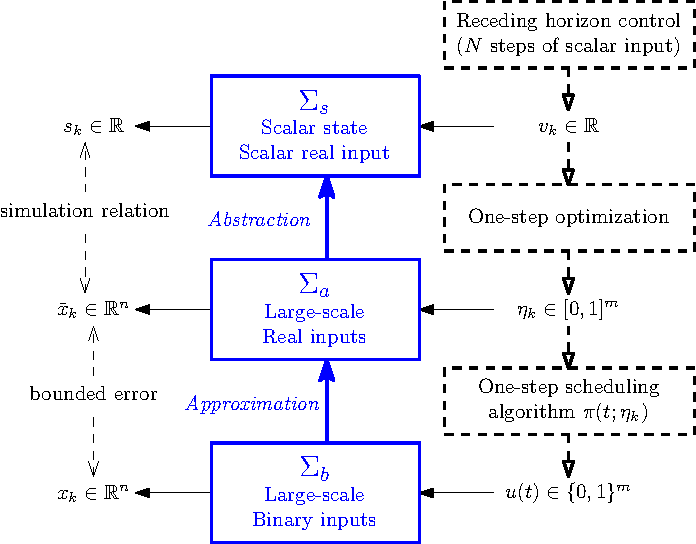
\includegraphics[width=\columnwidth]{approach_overview}
  \caption{Overview of the approach.}
  \label{fig:overview}
\end{figure}


%%% Local Variables:
%%% mode: latex
%%% TeX-master: "emsoft15gs"
%%% End:


\section{Approximation by Averaging} % Averaged Systems}
\label{sec:averaged-system}

Consider the averaged system $\Sigma_a$ of $\Sigma_b$ for each time interval $t \in [kT, (k + 1) T)$: $\dot{\overbar{x}} (t) = A \overbar{x} (t) + B \eta_k + Ew (t)$.
Recall that the \emph{utilization} $\eta_k = \frac{1}{T} \int_{kT}^{(k + 1) T} u (\tau) \mathd \tau$ is the average value of $u(t)$ in the interval, and is a vector of real numbers in $[0, 1]$. % $\eta_k \in [0, 1]^m$.
Initially $\overbar{x}_{0} = \overbar{x} (0) = x(0)$.
Generally, as $k$ increases, $\overbar{x}_{k}$ may deviate further and further from $x (kT)$, which is undesirable since the state constraint $\XSet$ needs to be maintained at all time.
For this reason, as mentioned earlier, we reset the value of $\overbar{x}$ to the measured state $x$ at each time instant $kT$, to keep the deviation within a tight bound.
The deviation $e (t) = x (t) - \overbar{x} (t)$ follows the dynamics
\begin{math}
  \dot{e} (t) %= A (x (t) - \overbar{x} (t)) + B (u (t) - \eta_k) 
  = Ae (t) + B (u (t) - \eta_k) \label{eq:err-dynamics}
\end{math}
for all $t \in [kT, (k + 1) T)$ and $e (kT) = 0$.
At the next instant $(k + 1) T$, the error is given by the solution of this differential equation: %, which is %~\eqref{eq:err-dynamics}
\begin{equation*}
e_{k+1} = e ((k + 1) T) = \int_{kT}^{(k + 1) T} \mathe^{A ((k + 1) T - s)} B (u (s) - \eta_k) \mathd s \text.
\end{equation*}
A tight bound on $e_{k+1}$ can be obtained, which is dependent on the value of $\eta_k$.
In this section, we make a practical assumption that the
state matrix $A$ is diagonalizable with real eigenvalues, that is $VA = DV$
where $D$ is a diagonal matrix of the eigenvalues of $A$ and $V$ is a non-singular matrix whose columns are the corresponding right eigenvectors.
%Many practical systems, especially in our targeted energy applications, this assumption is satisfied.
We can then transform the state with $V$ by defining a new state $z = Vx$, whose dynamics are
\[ \dot{z} = V \dot{x} = VAx + VBu + VEw = Dz + VBu + VEw \text.\]
%and which is subject to state constraint $z (t) \in V\mathcal{X}$.
This new model is in the form of $(\Sigma_b)$ with a diagonal state matrix.
%As a consequence, we can assume without loss of generality that the original system $\Sigma_b$ has diagonal state matrix $A$ because otherwise, we can always equivalently transform $\Sigma_b$ to achieve this.
Let $\lambda_i$ be the $i$-th diagonal element of $D$, for $i = 1, \ldots, n$.
The following theorem provides bounds on $e_{k+1}$, which depend on $\eta_{k}$.

\begin{theorem}
  \label{thm:averaged-sys-bound}
  Let $b_i$ be the $i^{\text{th}}$ row of $VB$, $\overbar{b}_i \geqslant 0$ the sum of all positive elements of $b_i$, and $\underline{b}_i \leqslant 0$ the sum of all negative elements of $b_i$.
  For each $i = 1,\ldots,n$, define
  \[ \xi_i =
  \begin{cases}
    0 & \text{if $\lambda_{i} = 0$} \\
    \frac{1}{\lambda_i} (\mathe^{\lambda_i T} - 1) - T & \text{if $\lambda_i > 0$}\\
    \frac{1}{\lambda_i} (\mathe^{\lambda_i T} - 1) - T \mathe^{\lambda_i T} & \text{if $\lambda_i < 0$}
  \end{cases} \]
  and $\overbar{\varepsilon}_{i} = \xi_{i} \overbar{b}_{i}$, $\underline{\varepsilon}_{i} = \xi_{i} \underline{b}_{i}$.
  Define $\tilde{B} = V^{-1} \Xi B$ where $\Xi$ is the diagonal matrix of all $\xi_{i}$.
  Then the error $e_{k+1}$ is bounded by
  \begin{equation*}
    \underline{\varepsilon} \leqslant V (e_{k+1} + \tilde{B} \eta_{k}) \leqslant \overbar{\varepsilon} \quad \text{(element-wise)}
  \end{equation*}
  where $\overbar{\varepsilon}$ and $\underline{\varepsilon}$ are the vectors of all $\overbar{\varepsilon}_{i}$ and $\underline{\varepsilon}_{i}$ respectively.
  Equivalently, $e_{k+1} = \varepsilon - \tilde{B} \eta_{k}$ for some $\varepsilon$ bounded element-wise by $\underline{\varepsilon} \leqslant \varepsilon \leqslant \overbar{\varepsilon}$.
\end{theorem}

  % OLD CONTENT OF THEOREM WITHOUT V
  % Consider each element $e_i ((k + 1) T)$ of the
  % error $e ((k + 1) T)$, $1 \leqslant i \leqslant n$. If $a_i = 0$ then $e_i
  % ((k + 1) T) = 0$. Otherwise, $e_i ((k + 1) T)$ is bounded by
  % \[ \xi_i  (\underline{\varepsilon}_i - b_i \eta_k) = \underline{e}_i
  %    (\eta_k) \leqslant e_i ((k + 1) T) \leqslant \overbar{e}_i (\eta_k) =
  %    \xi_i  (\overbar{\varepsilon}_i - b_i \eta_k) \]
  % for all $u (t)$ such that $\eta_k = \frac{1}{T} \int_{kT}^{(k + 1) T} u (t)
  % \mathd t$, where $b_i$ is the $i^{\text{th}}$ row of $B$,
  % $\overbar{\varepsilon}_i$ is the sum of all positive elements of $b_i$,
  % $\underline{\varepsilon}_i$ is the sum of all negative elements of $b_i$,
  % and
  % \[ \xi_i = \left\{ \begin{array}{ll}
  %      \frac{1}{a_i} (\mathe^{a_i T} - 1) - T & \text{if } a_i > 0\\
  %      \frac{1}{a_i} (\mathe^{a_i T} - 1) - T \mathe^{a_i T} & \text{if } a_i
  %      < 0
  %    \end{array} \right._{} \]


% The bound range $[\underline{e}_i (\eta_k), \overbar{e}_i (\eta_k)]$ given by
% \cref{thm:averaged-sys-bound} expands as $T$
% increases. Therefore, as $k$ increases, $\overbar{x} (kT)$ may
% deviate further and further from $x (kT)$, which is undesirable when the state
% constraint needs to be maintained. For this reason, to keep the deviation
% within a tight bound, we reset the state $\overbar{x}$ of $\Sigma_a$ to the
% measured state $x$ of $\Sigma_b$ at each $kT$, so that $e (kT)$ is reset to
% $0$. 
% Because $\overbar{x}_{k}$ is reset to $x(kT)$ at each time instant $k T$, the difference $e_{k+1}$ between $x ((k + 1) T)$ and the next value of
% $\overbar{x} (k)$ under $\eta_k$ is always bounded in $[\underline{e}_i
% (\eta_k), \overbar{e}_i (\eta_k)]$ for all $k$.

The proof can be found in \cref{sec:proof:averaged-sys-bound}.
We note that the utilization $\eta_{k}$, \ie the control input of $\Sigma_{a}$, enters affinely in the bounds on $e_{k+1}$.

\begin{remark}
We can still use our approach when $A$ is not
diagonalizable, however the error bounds obtained in
\cref{thm:averaged-sys-bound} must be generalized. For instance, we can
use the Jordan normal form to transform $A$ into a block diagonal
matrix, and obtain bounds in a way similar to that in
\cref{thm:averaged-sys-bound}. The made assumption simplifies the
presentation of our results but does not limit the practicality of our
approach. % much because, as we mentioned, many practical applications satisfy the assumption.
\end{remark}

%%% Local Variables:
%%% mode: latex
%%% TeX-master: "emsoft15gs"
%%% End:


\section{Model Abstractrion with Simulation Relations}
\label{sec:abstraction}

As we discussed in \cref{sec:overview}, to further reduce the optimization program~\eqref{eq:averaged-optim}, we employ the notion of model abstraction and simulation relations.
We first distinguish model abstraction and model order reduction.
Model order reduction is a common technique in control theory to reduce the order of a large-scale system so that it becomes manageable. The reduced model, however, still has
the same input and output as the original model. Under the same input signal,
the reduced model should produce an output signal which approximates that of
the original model, within some error bound. The left diagram in
\cref{fig:reduction-vs-abstraction} illustrates this concept, where
$\mathcal{M}_2$ is a reduced-order model of $\mathcal{M}_1$. On the other
hand, model abstraction derives a new model, usually of a lower order, with
completely different input and output than the original model. However, there
exists a relation between the states of the two models that can be maintained
along their evolutions. In other words, one model can track the behavior of
the other under this relation. The right diagram in
\cref{fig:reduction-vs-abstraction} depicts two models with a symbolic
relation $\mathcal{R}$ between their states. If for any admissible input $u_2
(\cdot)$ to $\mathcal{M}_2$ there exists an admissible input $u_1 (\cdot)$ to
$\mathcal{M}_1$ so that the state relation is always maintained along the
traces of the two models, we have a model abstraction. Furthermore, we may
require that a symbolic relation $\mathcal{R}_y$ between their outputs (observations) is also
maintained. A nice property of model abstraction is that we can design a
controller for $\mathcal{M}_1$ by first designing a supposedly simpler
controller for $\mathcal{M}_2$ and then refining it for $\mathcal{M}_1$ using
the symbolic state relation.

\begin{figure}[tb]
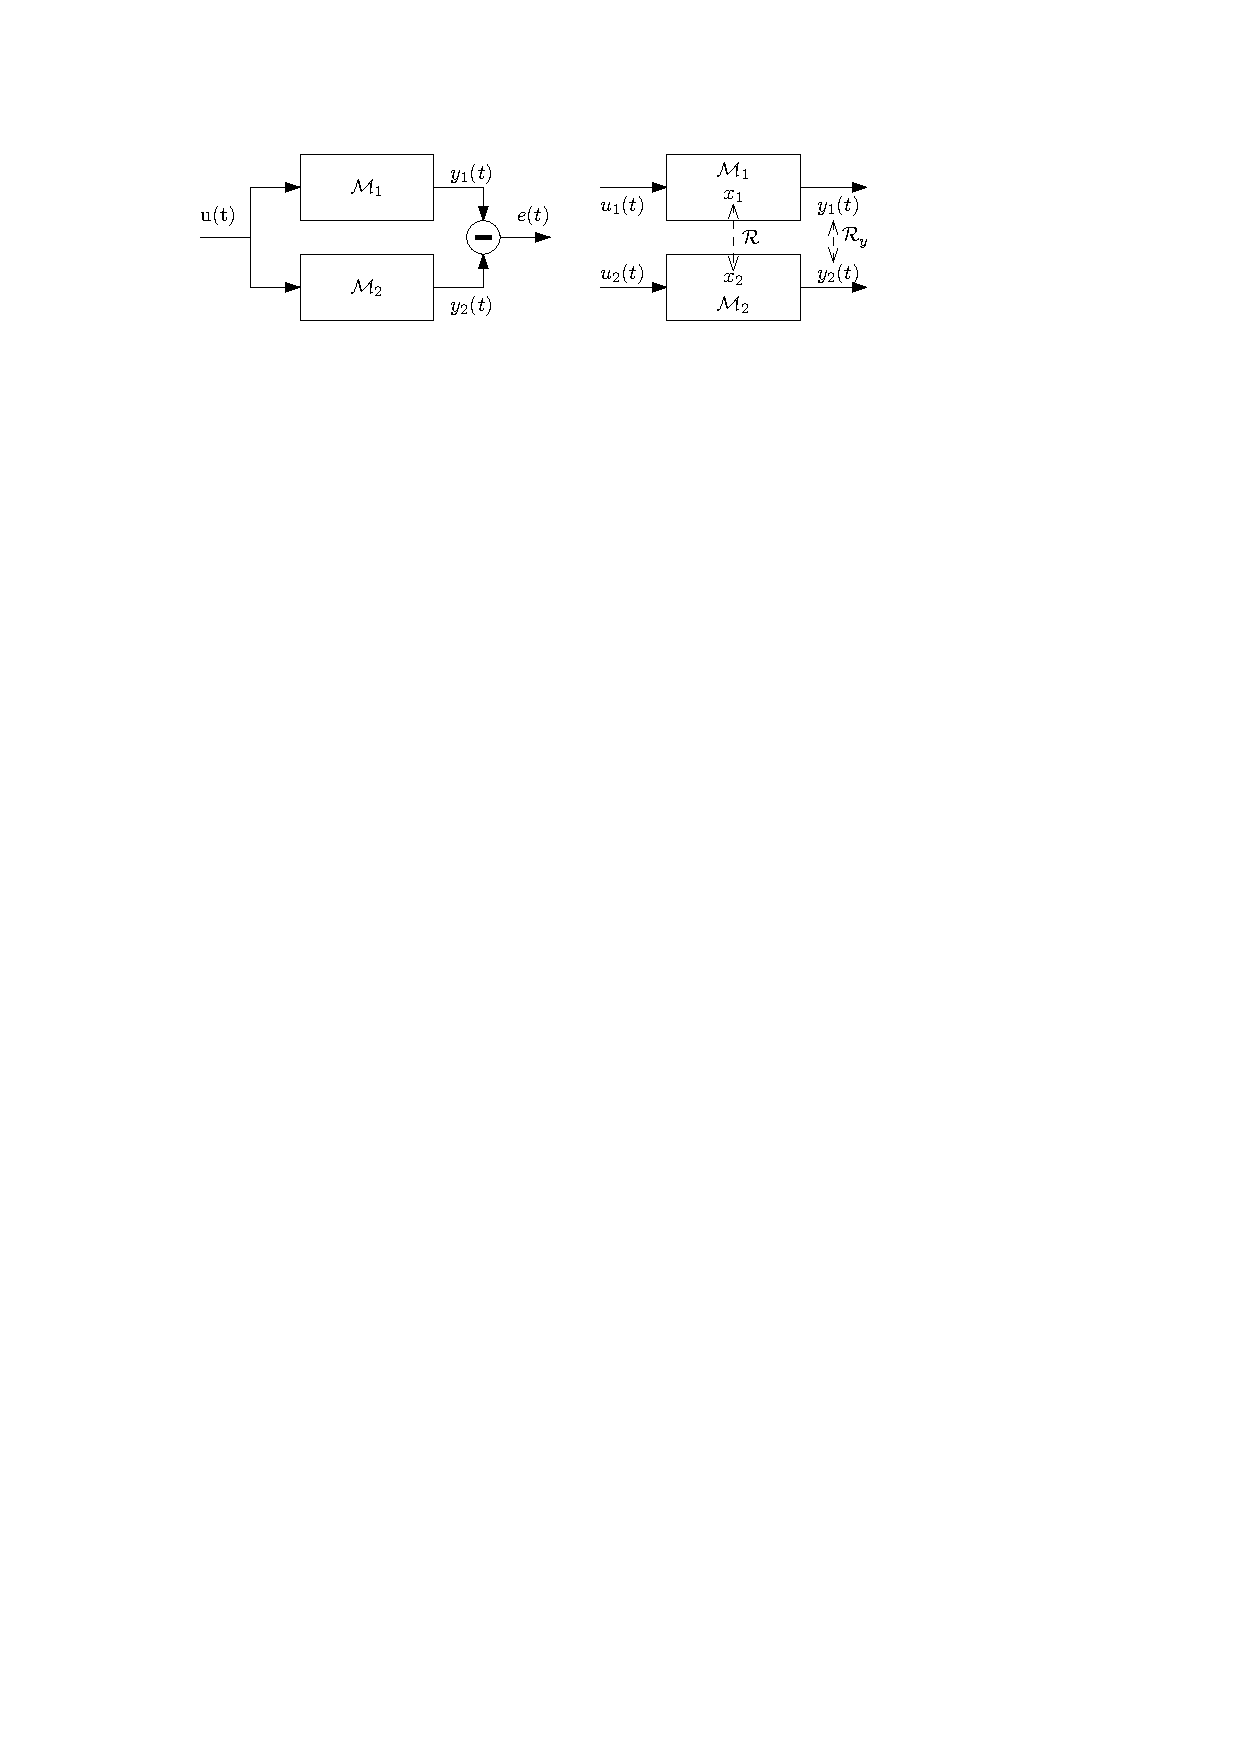
\includegraphics[width=\columnwidth]{abstraction_vs_reduction}
\caption{\label{fig:reduction-vs-abstraction}Model abstraction (right) is
  different from model order reduction (left): the models $\mathcal{M}_{1}$ and $\mathcal{M}_{2}$ do not share the same inputs nor outputs; instead they maintain a relation between their states along their evolutions.}
        \vspace{-10pt}
\end{figure}

\subsection{Simulation Relations} % Transition Systems}
\label{sec:abstraction:simulation}

In this section we review the concept of simulation relations between
transition systems. The readers are referred to \cite{girardetal07amd,aluretal00dah} for more thorough treatments of the subject.

The framework of transition systems allows us to unify the modeling of
discrete and continuous, deterministic and non-deterministic dynamical
systems. As we do not concern with the observable outputs of the systems in
this paper, we remove the observation aspect from the definition of transition
systems in {\cite{girardetal07amd}}:
      \vspace{-5pt}
\begin{definition}[Transition System, {\cite{girardetal07amd}}]
  \label{thm:transition-systems-def}
  A transition system is a tuple $T = (Q, \Sigma, \rightarrow, Q^0)$ that
  consists of
        \vspace{-5pt}
  \begin{itemize}
  \item a possibly infinite set $Q$ of states;
      \vspace{-5pt}
  \item a possibly infinite set $\Sigma$ of labels;
      \vspace{-5pt}
  \item a transition relation $\rightarrow \subseteq Q \times \Sigma \times
    Q$;
          \vspace{-5pt}
  \item a possibly infinite set $Q^0 \subseteq Q$ of initial states.
  \end{itemize}
\end{definition}

A transition from state $q$ to state $q^+$ under the label $\sigma$, {\ie}
$(q, \sigma, q^+) \in \rightarrow$, is denoted $q \xrightarrow{\sigma} q^+$.
We assume that the transition systems are {\emph{nonblocking}}, meaning that
for all $q \in Q$, there exists at least one transition starting from $q$. If
for any $q \in Q$ and any $\sigma \in \Sigma$, there is at most one transition
$q \xrightarrow{\sigma} q^+$ of $T$ and $Q^0$ is a singleton, then $T$ is
called {\emph{deterministic}}. Otherwise, it is called
{\emph{nondeterministic}}.

\begin{example}
  The framework of transition systems generalizes dynamical systems. As an
  example, consider a nonlinear discrete-time dynamical system $x^+ = f (x,
  u)$ where $x \in \mathbbm{R}^n$ is the state and $u \in \mathbbm{R}^m$ is
  the input, with initial state $x_{0}$.
  This system can be represented by a deterministic transition
  system $T$ with $Q =\mathbbm{R}^n$, $\Sigma =\mathbbm{R}^m$,
  $\rightarrow = \{ (x, u, x^+) |x \in Q, u \in \Sigma, x^+ = f (x, u) \in Q
  \}$, and $Q^{0} = \{x_{0}\}$.
  If the system is subject to disturbance: $x^+ = f (x, u, w)$ where
  $w \in \mathcal{W} \subseteq \mathbbm{R}^p$ is the disturbance, then $T$
  becomes nondeterministic where $\rightarrow = \{ (x, u, x^+) |x \in Q, u \in
  \Sigma, w \in \mathcal{W}, x^+ = f (x, u, w) \in Q \}$.
\end{example}

A simulation relation between two transition systems $T_1 = (Q_1, \Sigma_1,
\rightarrow_1, Q^0_1)$ and $T_2 = (Q_2, \Sigma_2, \rightarrow_2, Q^0_2)$ is a
stronger notion of system refinement, which allows one system to ``track'' the
other system while maintaining a certain relation between their states.
%A simulation relation is defined in \cref{def:simulation-relation}.

\begin{definition}[Simulation]
  \label{def:simulation-relation}A relation $\mathcal{R} \subseteq Q_1 \times
  Q_2$ is called a simulation relation of $T_1$ by $T_2$ if and only if for all $(q_1,
  q_2) \in \mathcal{R}$ and for all transitions $q_1 \xrightarrow{\sigma_1}_{1}
  q^+_1$, there exists a transition $q_2 \xrightarrow{\sigma_2}_{2}
  q^+_2$ such that $(q_1^+, q_2^+) \in \mathcal{R}$.
\end{definition}

Note that in \cite{girardetal07amd}, %it is required that
$T_1$ and $T_2$ have the same
label sets and $\sigma_{1} = \sigma_2 = \sigma$, % and the same observation sets),
however in \cref{def:simulation-relation} we %modify the definition to
relax this requirement, \ie $\Sigma_1$ and $\Sigma_2$, hence $\sigma_{1}$ and $\sigma_{2}$, can be different.
$T_2$ is said to simulate $T_1$, denoted $T_1 \preceq T_2$, if there exists a
simulation relation $\mathcal{R}$ of $T_1$ by $T_2$ such that for all $q_1 \in
Q^0_1$, there exists $q_2 \in Q^0_2$ such that $(q_1, q_2) \in \mathcal{R}$.
Intuitively, if $T_1 \preceq T_2$ then every state trajectory of $T_1$ can be
``tracked'' by $T_2$ with respect to the state relation $\mathcal{R}$.
Simulation relations and their variants are a powerful tool for safety verification and
hierarchical controller design \cite{clarkeetal99m,pappasetal00hcc,GirardEtAl06vus,girardetal07amd}.

\subsection{Input-Constrained Simulation Relations}
\label{sec:abstraction:ext-simulation}

Conventionally, simulation relations as defined in \cref{sec:abstraction:simulation} do not explicitly take into account %state constraints and
disturbances.  Moreover, there is no relation between the inputs (or labels) to the two systems as required for the total demand bound in our problem.  Therefore, this section extends the concept of simulation relations to account for these ingredients.

\begin{remark}
  For nondeterministic systems, the simulation relation as defined in
  \cref{def:simulation-relation} is not robust to the
  nondeterminism. In particular, it is implicitly assumed that the transition
  from any $q_1$ under any $\sigma_1$, although nondeterministic, is
  detectable so that an appropriate transition $q_2 \xrightarrow{\sigma_2}
  q^+_2$ can be selected. $T_2$ is not nondeterministic anymore because here
  $q_2 \xrightarrow{\sigma_2} q^+_2$ can be chosen to satisfy $(q_1^+, q_2^+)
  \in \mathcal{R}$. Furthermore, it assumes no correlation between the
  nondeterminism of the two systems. In reality, their nondeterminism may be
  correlated, for example if they are subject to the same disturbances in
  different ways. Our extended definition of simulation relations provides
  options for robustness to disturbances and nondeterminism correlation.
\end{remark}

\begin{remark}
  A relation between the labels of $T_1$ and $T_2$ generalizes the simulation
  relation definition in {\cite{girardetal07amd}}, where $\sigma_1$ and
  $\sigma_2$ are related by $\sigma_1 = \sigma_2$ (provided that $\Sigma_1 =
  \Sigma_2$).
\end{remark}

In this section, we generalize the label $\sigma$ of a transition system $T$ as a pair $\sigma = (\upsilon, \delta)$ of a control label $\upsilon \in \mathcal{U}$ and a disturbance label $\delta \in \mathcal{D}$.
Here, $\mathcal{U}$ and $\mathcal{D}$ are respectively the (possibly infinite) sets of control labels and disturbance labels.
The definition of the transition relation is modified accordingly as $\rightarrow \subseteq Q \times \mathcal{U} \times \mathcal{D} \times Q$, and a transition $(q, \upsilon, \delta, q^{+}) \in \rightarrow$ is denoted $q \xrightarrow{(\upsilon, \delta)} q^{+}$.
%The label set $\Sigma$ in \cref{thm:transition-systems-def} is the product $\mathcal{U} \times \mathcal{D}$.
%A transition system is also augmented with a state constraint $Q^S \subseteq Q$ and a mixed constraint $\mathcal{Y} \subseteq Q \times \mathcal{U}$.
Given two transition systems $T_{1}$ and $T_{2}$, we impose a constraint between their control labels $\upsilon_{1}$ and $\upsilon_2$ as a relation $\mathcal{R}_u \subseteq \mathcal{U}_1 \times \mathcal{U}_2$, and a constraint between their disturbance labels $\mathcal{R}_{d}\subseteq \mathcal{D}_1 \times \mathcal{D}_2$.
Note that the constraint $\mathcal{R}_{u}$ is desirable but not required for the execution of the transition systems, \ie an admissible execution of the transition systems may violate the constraint.
The relation $\mathcal{R}_{d}$ takes effect whenever $T_{1}$ and $T_{2}$ are executed simultaneously in the same environment.
%In the following, $\mathcal{P}^{+}(S)$ denotes the set of all non-empty subsets of a set $S$, \ie the superset of $S$ excluding $\emptyset$.
For system $T_{i}$, the set of all admissible successor states from a state $q_{i}$ under label $\sigma_{i} = (\upsilon_{i}, \delta_{i})$ is denoted by $\operatorname{succ}_{i}(q_{i}, \upsilon_{i}, \delta_{i}) = \{q_{i}^{+} \,|\, (q_{i}, \upsilon_{i}, \delta_{i}, q_{i}^{+}) \in \rightarrow_{i}\}$.

\begin{definition}[Input-constrained Simulation]
  \label{thm:ex-simulation-relation}
  % A pair $(\mathcal{R}, \mathcal{R}_{c}$ of a relation $\mathcal{R} \subseteq Q^{S}_1 \times Q^{S}_2$ and a map $\mathcal{R}_{c}: \mathcal{U}_{2} \to \mathcal{P}^{+}(\mathcal{R})$ 
  A relation $\mathcal{R} \subseteq Q^{S}_1 \times Q^{S}_2$ is an input-constrained simulation relation of $T_1$ by $T_2$ if and only if for all $(q_1, q_2) \in \mathcal{R}$ and all $(\upsilon_{1}, \delta_{1}) \in \mathcal{U}_{1} \times \mathcal{D}_{1}$ such that $\operatorname{succ}_{1} (q_{1}, \upsilon_{1}, \delta_{1}) \neq \emptyset$, there exists $\upsilon_{2} \in \mathcal{U}_{2}$ such that
    \begin{enumerate}
    \item $(\upsilon_{1}, \upsilon_{2}) \in \mathcal{R}_{u}$; and
    \item for all $\delta_{2} \in \mathcal{D}_{2}$ such that $(\delta_{1}, \delta_{2}) \in \mathcal{R}_{d}$, $\operatorname{succ}_{2} (q_{2}, \upsilon_{2}, \delta_{2}) \neq \emptyset$ and $(q_{1}^{+}, q_{2}^{+}) \in \mathcal{R}$ %_{c}(\upsilon_{2})$
      $\forall (q_{1}^{+}, q_{2}^{+}) \in \operatorname{succ}_{1} (q_{1}, \upsilon_{1}, \delta_{1}) \times \operatorname{succ}_{2} (q_{2}, \upsilon_{2}, \delta_{2})$.
    \end{enumerate}
\end{definition}


The existence of an input-constrained simulation relation $\mathcal{R}$ of $T_{1}$ by $T_{2}$ allows $T_{2}$ to track any state sequence of $T_{1}$ with respect to $\mathcal{R}$, as long as their initial states are in $\mathcal{R}$.
We define a trajectory of $T_{i}$ as a (potentially infinite) sequence of admissible states, labels, and transitions: $q_{i}^{0} \xrightarrow{\upsilon_{i}^{0}, \delta_{i}^{0}}_{i} q_{i}^{1} \xrightarrow{\upsilon_{i}^{1}, \delta_{i}^{1}}_{i} q_{i}^{2} \cdots$.
The next lemma follows directly from the \cref{thm:ex-simulation-relation}.
It essentially says that if an input-constrained simulation relation $\mathcal{R}$ of $T_{1}$ by $T_2$ exists then $T_{2}$ can be controlled to track any admissible trajectory of $T_{1}$, with respect to $\mathcal{R}$, while keeping the input constraint $\mathcal{R}_{u}$.

\begin{lemma}
  \label{thm:ex-simulation-tracking}
  Suppose $\mathcal{R}$ is an input-constrained simulation relation of $T_{1}$ by $T_{2}$, whose initial states satisfy $(q_{1}^{0}, q_{2}^{0}) \in \mathcal{R}$.
  Let $\kappa_{2}: Q_{1} \times \mathcal{U}_{1} \times \mathcal{D}_{1} \times Q_{2} \to \mathcal{U}_{2}$ be any feedback law such that for all admissible quadruples $(q_{1}, \upsilon_{1}, \delta_{1}, q_{2}) \in Q_{1} \times \mathcal{U}_{1} \times \mathcal{D}_{1} \times Q_{2}$, $\upsilon_{2} = \kappa_{2} (q_{1}, \upsilon_{1}, \delta_{1}, q_{2})$ satisfies the conditions in \cref{thm:ex-simulation-relation}.
  Such a feedback law always exists.
  Then for any trajectory of $T_{1}$, %(respectively, $\upsilon_{2}^{k} = \rho_{2} (q_{1}^{k}, \upsilon_{1}^{k}, q_{2}^{k})$)
  any corresponding trajectory of $T_{2}$ with $\upsilon_{2}^{k} = \kappa_{2} (q_{1}^{k}, \upsilon_{1}^{k}, \delta_{1}^{k}, q_{2}^{k})$ satisfies $(q_{1}^{k}, q_{2}^{k}) \in \mathcal{R}$ and $(\upsilon_{1}^{k}, \upsilon_{2}^{k}) \in \mathcal{R}_{u}$ for all $k$.
\end{lemma}

%%% Local Variables:
%%% mode: latex
%%% TeX-master: "emsoft15gs"
%%% End:


\section{Model Abstraction for Energy System Scheduling}%Green\\Scheduling}
\label{sec:abstraction-gs}

Going back to the %green
energy system scheduling problem, we apply the framework of input-constrained simulation relations to abstract the high-dimensional model $\Sigma_{a}$ by a low-dimensional model $\Sigma_{s}$.
We then derive a feedback control law that allows $\Sigma_{a}$ to track the state of $\Sigma_{s}$ while maintaining their simulation relation, all their state and input constraints, as well as the input upper-bounds set by $\Sigma_{s}$.
In particular, we consider the scalar discrete-time system $\Sigma_{s}$:
\begin{align}
  (\Sigma_s) \quad
  & s_{k + 1} = \alpha s_k + v_k + \beta^T w_{k}   \label{eq:abstract-system} \\
  & s_k \in \SSet \subseteq \mathbbm{R},
  v_k \in \VSet \subseteq \mathbbm{R},
  (s_k, v_k) \in \Omega \subseteq \SSet \times \VSet \nonumber
 \end{align}
%
The intuition is that $s_{k}$ represents an aggregated state of all the subsystems at time step $k$ and $v_{k}$ specifies an upper-bound of the total energy demand.
For example, consider an energy system consisting of $n$ rooms and a heater in each room, where the heaters have fixed heating powers and can only be switched on and off.
At time $k$, $s_{k}$ can represent the total enthalpy of all rooms, while $v_{k}$ bounds the total heating energy of all heaters during that interval.
Because the system is subject to heat loss and disturbances, the dynamics of $s$ have the form of \eqref{eq:abstract-system}.

The abstraction of $\Sigma_{a}$, \ie the input-constrained simulation relation $\RSet$, depends on how the control input $v_{k}$ is computed and how the disturbances are represented in $\Sigma_{s}$.
In practice, forecasts of the disturbances, denoted $\tilde{w}_{k}$, with known bounded accuracies are often available and used in computing the control inputs for both $\Sigma_{s}$ and $\Sigma_{a}$.
The forecast accuracies are represented by a vector $\zeta \geq 0$ in $\mathbb{R}^{p}$ such that the error between $w_{k}$ and $\tilde{w}_{k}$ are always bounded element-wise as $-\zeta \leqslant w_{k} - \tilde{w}_{k} \leqslant \zeta$ for all $k$.

We consider two control approaches in this paper:
\begin{enumerate}
\item \textbf{Feedforward approach:} The control sequence $v_{0}$, $v_{1}$, \dots, $v_{N-1}$ of $\Sigma_{s}$ are computed using the disturbance forecasts $\tilde{w}_{0}, \tilde{w}_{1}, \dots, \tilde{w}_{N-1}$ as nominal disturbances for the horizon.  These control inputs are not adjusted until the end of the horizon; in other words, the control law for $\Sigma_{s}$ is feedforward.  Consequently, the trajectory of $\Sigma_{s}$ is nominal without taking into account actual disturbances.  The control input $\eta_{k}$ for $\Sigma_{a}$ is computed based on the actual state $\overbar{x}_{k}$ of $\Sigma_{a}$ and the nominal state, control, and disturbances of $\Sigma_{s}$, hence it is a feedback law.
\item \textbf{Feedback approach:} At each time step $k$, $v_{k}$ is decided using the actual state $s_{k}$, which is computed from the observed actual state $\overbar{x}_{k}$. %, and the disturbance forecast $\tilde{w}_{k}$.
  The state trajectory of $\Sigma_{s}$ is therefore actual, not nominal.  The control input $\eta_{k}$ is calculated from the actual states $s_{k}$ and $\overbar{x}_{k}$, and $v_{k}$ and $\tilde{w}_{k}$.  Hence, both control laws for $\Sigma_{a}$ and $\Sigma_{s}$ are feedback.
\end{enumerate}

%Assuming that the parameters $\alpha$ and $\beta$ of $\Sigma_{s}$ are given, 
We derive the abstraction $\Sigma_{s}$ of $\Sigma_{a}$ for each approach in three steps:
\begin{enumerate}
\item $\Sigma_{s}$ and $\Sigma_{a}$ are formulated as transition systems $T_{1}$ and $T_{2}$ respectively;
\item Assuming a certain form of $\RSet$, we derive %a necessary and sufficient
  conditions for $\RSet$ to be an input-constrained simulation relation;
\item Based on the conditions, we develop algorithms to compute the parameters of $\Sigma_{s}$, its joint constraint $\Omega$, and the simulation relation $\RSet$.
\end{enumerate}
%
%In \cref{sec:abstraction-gs:sigma-s} we will discuss how the parameters of $\Sigma_{s}$ are computed.


\subsection{Feedforward Approach}
\label{sec:abstraction-gs:feedforward}

\subsubsection{Transition Systems}
\label{sec:abstraction-gs:feedforward:Ts}

In the feedforward approach, the evolution of $\Sigma_{s}$ is nominal, where the (nominal) disturbances are known and deterministic.
We formulate $T_{1}$ as follows:
\begin{itemize}
\item State $q_{1} \equiv s$ and state set $Q_{1} = \mathcal{S}$.
\item Control label $\upsilon_{1} \equiv v$ with $\mathcal{U}_{1} = \mathcal{V}$.
\item Disturbance label $\delta_{1} \equiv \tilde{w}$ is the disturbance forecast with $\mathcal{D}_{1} = \WSet$ being the set of possible disturbances.
\item Transition set $\rightarrow_{1} = \{ (s, v, \tilde{w}, s^{+}) \,|\, (s,v) \in \Omega,\allowbreak \tilde{w} \in \WSet, %\mathcal{D}_{1},
  \allowbreak s^{+} = \alpha s + v + \beta^{T} \tilde{w} \in \SSet\}$. %Q_{1}
\end{itemize}
%
The transition system $T_{2}$ of $\Sigma_{a}$ is defined as:
\begin{itemize}
\item State is the averaged state $q_{2} \equiv \overbar{x}$ with $Q_{2} = \XSet$.
\item Control label $\upsilon_{2} \equiv \eta$ with $\mathcal{U}_{2} = [0,1]^{m}$.
\item Disturbance label: $\Sigma_{a}$ %the averaged system 
  is influenced by the actual disturbances $w_{k}$, therefore $\delta_{2} \equiv w$ with $\mathcal{D}_{2} = \WSet$.
\item Transition set: recall that at every time step $k+1$, $\overbar{x}_{k+1}$ is reset to $x((k+1)T)$, which is within a bounded error $e_{k+1}$ from $A_{T} \overbar{x}_{k} + B_{T} \eta_k + E_{T} w_{k}$ (\cf \cref{thm:averaged-sys-bound}).  This reset can be modeled as a non-deterministic but bounded perturbation of the state.  Therefore we define $\rightarrow_{2} = \{ (\overbar{x}, \eta, w, \overbar{x}^{+}) \,|\, \overbar{x} \in \XSet, \eta \in \mathcal{U}_{2}, w \in \WSet,\allowbreak \overbar{x}^{+} = A_{T} \overbar{x}+ B_{T} \eta + E_{T} w + e \in \XSet,\allowbreak 
\underline{\varepsilon} \leqslant V (e + \tilde{B} \eta) \leqslant \overbar{\varepsilon}\}$.
\end{itemize}
%
Because $v_{k}$ specifies an upper-bound of the total energy demand $T \rho^{T} \eta_{k}$, we define the joint input constraint $\RSet_{u} = \{ (v, \eta) \in \mathcal{U}_{1} \times \mathcal{U}_{2} \,|\, T \rho^{T} \eta \leq v \}$.
Finally, the forecast accuracy between nominal $\tilde{w}$ of $\Sigma_{s}$ and actual $w$ of $\Sigma_{a}$ is modeled by the disturbance relation $\RSet_{d} = \{ (\tilde{w}, w) \in \mathcal{D}_{1} \times \mathcal{D}_{2} \,|\, -\zeta \leqslant w - \tilde{w} \leqslant \zeta \}$.


\subsubsection{Conditions for \RSet} % Input-constrained Simulation Relation \protect\RSet}
\label{sec:abstraction-gs:feedforward:conditions}

To derive the model abstraction of $\Sigma_{a}$, the input-constrained simulation relation $\RSet$ must be computed.
Specifically, we need to be able to certify if any given relation $\RSet$ of $s$ and $\overbar{x}$ is an input-constrained simulation relation of $T_{1}$ by $T_{2}$.
The following theorem provides such a necessary and sufficient condition for $\RSet$.
Here, the product between a matrix $M \in \mathbb{R}^{m \times n}$ and a set $\PSet \subseteq \mathbb{R}^{n}$ is defined as the image of $\PSet$ under the linear map $M$, \ie $M \PSet = \{ y \in \mathbb{R}^{m} \,|\, y = M x, x \in \PSet\}$.
The identity matrix is denoted by $\IdentityMatrix$, whose dimensions are often omitted when they are obvious from the context.
The symbol $\Zero$ denotes a zero vector or matrix.

\begin{theorem}
  \label{thm:abstraction-gs:necessary-sufficient}
  A set $\RSet \subseteq \SSet \times \XSet$ is an input-constrained simulation relation of $T_{1}$ by $T_{2}$ for the feedforward approach if and only if
  \begin{align}
    \label{eq:abstraction-gs:necessary-sufficient}
    M_l \PSet_l \subseteq M_r \PSet_r
  \end{align}
  where 
  \begin{gather*}
    M_l =
          \begin{bmatrix}
            0 & \Zero & 1 & \Zero & \Zero & \Zero \\
            \alpha & \Zero & 1 & \Zero & \beta^{T} & \Zero \\
            0 & A_T & 0 & E_T & E_T & \IdentityMatrix
          \end{bmatrix}\\
    M_r =
      \begin{bmatrix}
        0 & \Zero & 1 & \Zero \\
        1 & \Zero & 0 & \Zero \\
        0 & \IdentityMatrix & 0 & \tilde{B} - B_{T}
      \end{bmatrix}
  \end{gather*}
  and
  \begin{align*}
    \PSet_l =& \big\{ (s,\overbar{x}, v, \delta, \tilde{w}, \varepsilon) \,\big|\,
              (s,\overbar{x}) \in \RSet,\ (s,v) \in \Omega, -\zeta \leqslant \delta \leqslant \zeta,\big.\\
            &\qquad \big. \tilde{w} \in \WSet, \tilde{w} + \delta \in \WSet, \alpha s + v + \beta^{T} \tilde{w} \in \SSet, \underline{\varepsilon} \leqslant \varepsilon \leqslant \overbar{\varepsilon} \big\} \\
    \PSet_r =& \big\{(s^+, \overbar{x}^{+}, \overbar{v}, \eta) \,\big|\,
               \overbar{x}^{+} \in \XSet, (s^{+}, \overbar{x}^{+}) \in \RSet, \eta \in [0,1]^{m},\big.\\
             &\qquad \big. T \rho^{T} \eta \leqslant \overbar{v}\big\}
  \end{align*}
\end{theorem}
The proof can be found in \cref{sec:proof:abstraction-gs:necessary-sufficient}.

Although \cref{thm:abstraction-gs:necessary-sufficient} is useful for verifying whether a given $\RSet$ is an input-constrained simulation relation, it does not allow us to directly compute $\RSet$ since $\RSet$ appears on both sides of \eqref{eq:abstraction-gs:necessary-sufficient}.
Furthermore, computing the image of a set under a linear map and checking for a set inclusion are generally difficult.
Therefore, we will impose a certain structure on the relation $\RSet$ that results in polyhedral sets $\PSet_{l}$ and $\PSet_{r}$.
We will also derive a simpler condition for $\RSet$, which can be verified by checking the feasibility of a linear program.

As mentioned in the overview in \cref{sec:overview} and again at the beginning of this section, $s$ represents an aggregated state of all the subsystems, for example the total enthalpy of an energy system.
Thus, we can choose $s$ to be approximately a linear combination of all the (energy) states of the subsystems.
Let $s \approx c^{T} \overbar{x}$, where $c$ is a constant vector in $\mathbb{R}^{n}$.
The set $\RSet$ is chosen to represent this relationship between $s$ and $\overbar{x}$ as 
\begin{equation}
  \label{eq:abstraction-gs:R}
  \RSet = \{ (s,\overbar{x}) \in \SSet \times \XSet \,|\, | c^{T} \overbar{x} - s | \leqslant \gamma \} \text,
\end{equation}
where $\gamma \geqslant 0$ is a design parameter.
Intuitively, in an energy system, the set of $\overbar{x} \in \XSet$ such that $(s,\overbar{x}) \in \RSet$, for any $s \in \SSet$, is the set of all states that have roughly the same aggregated energy level $s$ (up to an error of $\gamma$).

We have assumed in \cref{sec:gs-problem} that $\XSet$ and $\WSet$ are polyhedra.
Suppose also that $\Omega$ is a polyhedron.
Let their hyperplane representations be
\begin{gather*}
  \XSet = \{ x \in \mathbb{R}^{n} \,|\, H_{x} x \leqslant k_{x} \}, \qquad
  \WSet = \{ w \in \mathbb{R}^{p} \,|\, H_{w} x \leqslant k_{w} \}\\
  \Omega = \{ (s,v) \in \SSet \times \VSet \,|\, H_{\Omega}^{s} s + H_{\Omega}^{v} v \leqslant k_{\Omega} \}
\end{gather*}
where $H_{x}$, $k_{x}$, $H_{w}$, $k_{w}$, $H_{\Omega}^{s}$, $H_{\Omega}^{v}$, $k_{\Omega}$ are matrices and vectors of appropriate dimensions.
Because $s$ and $v$ are scalars, we can bound them as $\underline{s} \leqslant s \leqslant \overbar{s}$ and $\underline{v} \leqslant v \leqslant \overbar{v}$, where $\underline{s}$, $\overbar{s}$, $\underline{v}$, $\overbar{v}$ are respectively the lower- and upper-bounds of $s$ and $v$.
Note that $\Omega$ is a subset of $\SSet \times \VSet = [\underline{s},\overbar{s}] \times [\underline{v},\overbar{v}]$.
With these assumptions, $\PSet_{l}$ and $\PSet_{r}$ become polyhedral sets.
We can now state a sufficient condition for $\RSet$ in the next theorem.

\begin{theorem}
  \label{thm:abstraction-gs:sufficient-LP}
  A set $\RSet$ as defined in \eqref{eq:abstraction-gs:R} is an input-constrained simulation relation of $T_{1}$ by $T_{2}$ for the feedforward approach if there exist a real matrix $Z$ of non-negative elements, a real matrix $Q$, and a real vector $q$ such that
  \begin{subequations}
    \label{eq:abstraction-gs:sufficient-LP}
    \begin{align}
      M_{r} Q &= \IdentityMatrix \\
      M_{r} q &= \Zero \\
      Z H_{l} &= H_{r} Q M_{l} \\
      Z k_{l} &\leqslant k_{r} - H_{r} q
    \end{align}
  \end{subequations}
  in which
  \begin{gather*}
    H_{l} =
    \left[ \begin{smallmatrix}
      %1 \\ %  & \Zero  &  \Zero
      %-1 \\ % & \Zero  &  \Zero
        & H_{x} \\ % &  \Zero
      -1  & c^{T} \\ % &  \Zero
      1   & -c^{T} \\ % &  \Zero
      H_{\Omega}^{s} & & H_{\Omega}^{v} \\
      %& & 1 \\
      %& & -1 \\
      & & & & H_{w} \\
      & & & H_{w} & H_{w} \\
      & & & \IdentityMatrix \\
      & & & -\IdentityMatrix \\
      \alpha & & 1 & & \beta^{T} \\
      -\alpha & & -1 & & -\beta^{T} \\
      & & & & & V \\
      & & & & & -V
    \end{smallmatrix} \right], \;
    k_{l} =
    \left[ \begin{smallmatrix}
      %\overbar{s} \\
      %-\underline{s} \\
      k_{x} \\
      \gamma \\
      \gamma \\
      k_{\Omega} \\
      %\overbar{v} \\
      %-\underline{v} \\
      k_{w} \\
      k_{w} \\
      \zeta \\
      \zeta \\
      \overbar{s} \\
      -\underline{s} \\
      \overbar{\varepsilon} \\
      -\underline{\varepsilon}
    \end{smallmatrix} \right] \\
    %
    H_{r} =
    \left[ \begin{smallmatrix}
      & H_{x} \\ % &  \Zero
      -1  & c^{T} \\ % &  \Zero
      1   & -c^{T} \\ % &  \Zero
      & & -1 & T \rho^{T} \\
      & & & \IdentityMatrix \\
      & & & -\IdentityMatrix
    \end{smallmatrix} \right], \;
    k_{r} =
    \left[ \begin{smallmatrix}
      k_{x} \\
      \gamma \\
      \gamma \\
      0 \\
      \One \\
      \Zero
    \end{smallmatrix} \right] \text.
  \end{gather*}
\end{theorem}
In the above matrices and vectors, the blank spaces are zero blocks and $\One$ denotes vector of 1's.
The theorem is proved in \cref{sec:proofs:abstraction-gs:sufficient-LP}.

Although \cref{thm:abstraction-gs:sufficient-LP} is only sufficient, it reduces the condition to checking the feasibility of the linear program~\eqref{eq:abstraction-gs:sufficient-LP}, which can be solved rather efficiently by any LP solver such as Gurobi, MOSEK, CPLEX, CLP.

We note that the design parameters, which are ($\alpha$, $\beta$, $c$, $\gamma$, $H_{\Omega}^{s}$, $H_{\Omega}^{v}$, $k_{\Omega}$), are multiplied by the elements of $Z$ in \eqref{eq:abstraction-gs:sufficient-LP}.
Consequently, if we want to solve \eqref{eq:abstraction-gs:sufficient-LP} to also find the design parameters, the problem becomes a bilinear program, which is intractable to solve for any significant size.
We will discuss a way to compute these parameters in \cref{sec:abstraction-gs:computation}, after we derive similar results for the feedback control approach in the next section.

\subsection{Feedback Approach}
\label{sec:abstraction-gs:feedback}

\subsubsection{Transition Systems}
\label{sec:abstraction-gs:feedback:Ts}

In the feedback approach, the evolution of $\Sigma_{s}$ is not nominal as it is influenced by the actual disturbances, which are unknown but within known accuracies from their forecasts.
To model this phenomenon, we will include the disturbance forecasts in the control labels of both $T_{1}$ and $T_{2}$, while their disturbance labels are the errors between the forecasts and the actual disturbances.
Specifically, we define $T_{1}$ as follows:
\begin{itemize}
\item State $q_{1} \equiv s$ and state set $Q_{1} = \mathcal{S}$.
\item Control label $\upsilon_{1} \equiv (v, \tilde{w}_{1})$ with $\mathcal{U}_{1} = \VSet \times \WSet$.
\item Disturbance label $\delta_{1}$ is the disturbance forecast error $\delta_{1} = w - \tilde{w}_{1}$; $\mathcal{D}_{1} = \{ \delta_{1} \in \mathbb{R}^{p} \,|\, -\zeta \leqslant \delta_{1} \leqslant \zeta\}$.
\item Transition set $\rightarrow_{1} = \{ (s, v, \tilde{w}_{1}, \delta_{1}, s^{+}) \,|\, (s,v) \in \Omega,\allowbreak \tilde{w}_{1} \in \WSet,\allowbreak \delta_{1} \in \mathcal{D}_{1},\allowbreak \tilde{w}_{1} + \delta_{1} \in \WSet,\allowbreak s^{+} = \alpha s + v + \beta^{T} (\tilde{w}_{1} + \delta_{1}) \in \SSet\}$. %Q_{1}
\end{itemize}
%
The transition system $T_{2}$ of $\Sigma_{a}$ is defined as:
\begin{itemize}
\item State $q_{2} \equiv \overbar{x}$; $Q_{2} = \XSet$.
\item Control label $\upsilon_{2} \equiv (\eta, \tilde{w}_{2})$ with $\mathcal{U}_{2} = [0,1]^{m} \times \WSet$.
\item Disturbance label $\delta_{2}$ is also the forecast error; $\mathcal{D}_{2} = \{ \delta_{2} \in \mathbb{R}^{p} \,|\, -\zeta \leqslant \delta_{2} \leqslant \zeta\}$.
\item Transition set: we again model the state reset as a non-deterministic but bounded perturbation of $\overbar{x}$.   Define $\rightarrow_{2} = \{ (\overbar{x}, \eta, \tilde{w}_{2}, \delta_{2}, \overbar{x}^{+}) \,|\, \overbar{x} \in \XSet, \eta \in \mathcal{U}_{2}, \tilde{w}_{2} \in \WSet,\allowbreak \delta_{2} \in \mathcal{D}_{2},\allowbreak \tilde{w}_{2} + \delta_{2} \in \WSet,\allowbreak \overbar{x}^{+} = A_{T} \overbar{x}+ B_{T} \eta + E_{T} (\tilde{w}_{2} + \delta_{2}) + e \in \XSet,\allowbreak \underline{\varepsilon} \leqslant V (e + \tilde{B} \eta) \leqslant \overbar{\varepsilon}\}$.
\end{itemize}
%
The joint input constraint $\RSet_{u}$ needs to take into account that the disturbance forecasts are the same for $T_{1}$ and $T_2$, hence $\RSet_{u} = \{ ((v, \tilde{w}_{1}), (\eta, \tilde{w}_{2})) \in \mathcal{U}_{1} \times \mathcal{U}_{2} \,|\, T \rho^{T} \eta \leq v, \tilde{w}_{1} = \tilde{w}_{2} \}$.
Finally, because $T_{1}$ and $T_{2}$ are subject to the same actual disturbances, we define the disturbance relation $\RSet_{d} = \{ (\delta_{1}, \delta_{2}) \in \mathcal{D}_{1} \times \mathcal{D}_{2} \,|\, \delta_{1} = \delta_{2} \}$.

\subsubsection{Conditions for \RSet} % Input-constrained Simulation Relation \protect\RSet}
\label{sec:abstraction-gs:feedback:conditions}

The only differences between the feedback and feedforward approaches are that in the feedback approach: (a) the control input $v$ for $T_{1}$ must robustly drive $s$ to $\SSet$ regardless of the forecast error $\delta$; (b) $s$ is updated with the actual disturbance $\tilde{w} + \delta$.
Therefore, the necessary and sufficient condition in \cref{thm:abstraction-gs:necessary-sufficient} still holds for the feedback approach with modified matrix $M_{l}$ and set $\PSet_{l}$:
\begin{gather*}
  M_l =
  \begin{bmatrix}
    0 & \Zero & 1 & \Zero & \Zero & \Zero \\
    \alpha & \Zero & 1 & \beta^{T} & \beta^{T} & \Zero \\
    0 & A_T & 0 & E_T & E_T & \IdentityMatrix
  \end{bmatrix}\\
  \begin{aligned}
    \PSet_l =& \big\{ (s,\overbar{x}, v, \delta, \tilde{w}, \varepsilon) \,\big|\,
    (s,\overbar{x}) \in \RSet,\ (s,v) \in \Omega, -\zeta \leqslant \delta \leqslant \zeta,\big.\\
    &\qquad \big. \tilde{w} \in \WSet, \tilde{w} + \delta \in \WSet, \alpha s + v + \beta^{T} \tilde{w} \in \SSet \ominus \beta^{T} \mathcal{D}_{1},\\
    &\qquad \underline{\varepsilon} \leqslant \varepsilon \leqslant \overbar{\varepsilon} \big\}
  \end{aligned}
\end{gather*}
where $\ominus$ denotes the Pontryagin difference between two sets.
Similarly, ~\cref{thm:abstraction-gs:sufficient-LP} is still valid when $k_{l}$ is modified accordingly:
\begin{equation*}
    k_{l} =
    \left[ \begin{smallmatrix}
      %\overbar{s} \\
      %-\underline{s} \\
      k_{x} \\
      \gamma \\
      \gamma \\
      k_{\Omega} \\
      %\overbar{v} \\
      %-\underline{v} \\
      k_{w} \\
      k_{w} \\
      \zeta \\
      \zeta \\
      \overbar{s} - \max_{\delta \in [-\zeta, \zeta]} \beta^{T} \delta\\
      -\underline{s} + \min_{\delta \in [-\zeta, \zeta]} \beta^{T} \delta\\
      \overbar{\varepsilon} \\
      -\underline{\varepsilon} 
    \end{smallmatrix} \right]
  \end{equation*}


\subsection{Computation of Design Parameters}
\label{sec:abstraction-gs:computation}

The design parameters of the model abstraction, which we aim to compute, are ($\alpha$, $\beta$, $c$, $\gamma$, $H_{\Omega}^{s}$, $H_{\Omega}^{v}$, $k_{\Omega}$).
As mentioned above, they enter the sufficient condition~(\cref{eq:abstraction-gs:sufficient-LP}) in bilinear terms, hence it is intractable to compute them (optimally) using this condition.
In this section, we present a method to design these parameters in a suboptimal but tractable way.

\subsubsection{Computing $\alpha$, $\beta$, $c$}

We compute these parameters based on the intuition that $s$ is the aggregated state of all the subsystems: $s \approx c^{T} \overbar{x}$.
From the discrete-time dynamics of $\overbar{x}$ we have
\begin{equation*}
  s_{k+1} \approx c^{T} \overbar{x}_{k+1} = c^{T} A_{T} \overbar{x}_{k} + c^{T} B_{T} \eta_{k} + c^{T} E_{T} w_{k}
\end{equation*}
while at the same time 
\begin{equation*}
s_{k+1} = \alpha s_{k} + v_{k} + \beta^{T} w_{k} \approx \alpha c^{T} \overbar{x}_{k} + T \rho^{T} \eta_{k} + \beta^{T} w_{k} \text.
\end{equation*}
Matching the two equations, we aim to find $\alpha$ and $c$ so that
$c^{T} B_{T} = T \rho^{T}$
while minimizing $\| c^{T} A_{T} - \alpha c^{T} \|$, where $\|\cdot\|$ denotes some vector norm.
If $B_{T}$ is full row rank, $c$ can be uniquely computed by solving a linear equation, and the minimization becomes a simple unconstrained program.
If $B_{T}$ is not full row rank, $c$ and $\alpha$ can be found by solving the above nonlinear optimization, which can be made unconstrained by rewriting $c$ in terms of the basis vectors of the kernel of $B_{T}^{T}$.
We then calculate $\beta = E_{T}^{T} c$.


\subsubsection{Computing $\gamma$ and $\Omega$}

Once $\alpha$, $\beta$, and $c$ are chosen, we can compute the parameter $\gamma$ of the relation $\RSet$ and the constraint set $\Omega$ of $(s,v)$.
We first choose the ranges $[\underline{s}, \overbar{s}]$ and $[\underline{v}, \overbar{v}]$ of $s$ and $v$ that satisfy
\begin{gather*}
  \underline{s} \geqslant \min_{x \in \XSet} c^{T} x, \quad
  \overbar{s} \leqslant \max_{x \in \XSet} c^{T} x \\
  \underline{v} \geqslant \min_{\Zero \leqslant \eta \leqslant \One} T \rho^{T} \eta, \quad
  \overbar{v} \leqslant \max_{\Zero \leqslant \eta \leqslant \One} T \rho^{T} \eta
\end{gather*}
based on the relationships between $s$ and $\overbar{x}$, $v$ and $\eta$.
Because $X$ is bounded, $\underline{s}$ and $\overbar{s}$ are finite; and so are $\underline{v}$ and $\overbar{v}$.

Choosing $\gamma$ and $\Omega$ is difficult because $\gamma$ appears in both $k_{l}$ and $k_{r}$, and $\Omega$ is a set.
Obviously, it is unnecessary for $\gamma$ to be larger than $\overbar{s} - \underline{s}$ due to the relation $| c^{T} \overbar{x} - s | \leqslant \gamma$.
Therefore we can select any value between $0$ and $\overbar{s} - \underline{s}$ for $\gamma$, with the apparent intuition that as $\gamma$ gets smaller, the constraint between $s$ and $\overbar{x}$ becomes stricter, keeping $(s, \overbar{x}$ in $\RSet$ is more difficult, hence $\RSet$ is less likely an input-constrained simulation relation.
For $\Omega$, which is a subset of $[\underline{s}, \overbar{s}] \times[\underline{v}, \overbar{v}]$, the following result allows us to construct $\Omega$ from smaller sets.

\begin{lemma}
  \label{thm:abstraction-gs:omega-union}
  Suppose that all the parameters are fixed except for $\Omega$.
  Let $\Omega_{1}$ and $\Omega_{2}$ are two subsets of $[\underline{s}, \overbar{s}] \times[\underline{v}, \overbar{v}]$ and suppose that they satisfy the sufficient condition in \cref{thm:abstraction-gs:sufficient-LP}.
  Then their union $\Omega_{1} \cup \Omega_{2}$ satisfies the necessary and sufficient condition in \cref{thm:abstraction-gs:necessary-sufficient}.
\end{lemma}
This lemma can be proved by noting that $\Omega_{1}$ and $\Omega_{2}$ satisfy \cref{thm:abstraction-gs:necessary-sufficient}, and $\Omega$ appears only in the left-hand side of the set inclusion~(\cref{eq:abstraction-gs:necessary-sufficient}).
Using this result, we can check the sufficient condition in \cref{thm:abstraction-gs:sufficient-LP} for small sets, then construct the final $\Omega$ set from their union.
This algorithm is outlined below.
\begin{enumerate}
\item We first grid the finite intervals of $s$ and $v$ as $\underline{s} = s^{0} < s^{1} < \cdots < s^{l_{s}} = \overbar{s}$ and $\underline{v} = v^{0} < v^{1} < \cdots < v^{l_{v}} = \overbar{v}$.  This effectively grids the box $[\underline{s}, \overbar{s}] \times[\underline{v}, \overbar{v}]$ into $l_{s} l_{v}$ small cells.
\item For each cell $\Omega_{i,j} = [s^{i}, s^{i+1}] \times[v^{j}, v^{j+1}]$, for $0 \leqslant i \leqslant l_{s}-1$ and $0 \leqslant j \leqslant l_{v}-1$, check if it satisfies \cref{thm:abstraction-gs:sufficient-LP}.
\item Construct $\Omega$ as the union of all cells $\Omega_{i,j}$ that satisfy \cref{thm:abstraction-gs:sufficient-LP}.  If the projection of $\Omega$ onto $s$ covers the entire range $[\underline{s}, \overbar{s}]$ then take $\Omega$.  This is to ensure that we can always find an admissible control input $v$ for any valid value of $s$.  We can simplify $\Omega$ by a convex polyhedron contained in the union, from which $H_{\Omega}^{s}$, $H_{\Omega}^{v}$ and $k_{\Omega}$ are extracted.
\end{enumerate}

\begin{remark}
  The constructed set $\Omega$ may not satisfy \cref{thm:abstraction-gs:sufficient-LP} because the condition is only sufficient.
  However, $\Omega$ is valid because it satisfies the stronger necessary and sufficient condition in \cref{thm:abstraction-gs:necessary-sufficient}, due to \cref{thm:abstraction-gs:omega-union}.
\end{remark}


% \subsection{Parameters of \protect$\Sigma_{s}$}
% \label{sec:abstraction-gs:sigma-s}




%%% Local Variables:
%%% mode: latex
%%% TeX-master: "emsoft15gs"
%%% End:


%ACKNOWLEDGMENTS are optional
%\section{Acknowledgments}


%
% The following two commands are all you need in the
% initial runs of your .tex file to
% produce the bibliography for the citations in your paper.
\bibliographystyle{abbrv}
\bibliography{IEEEabrv,references}
% You must have a proper ".bib" file
%  and remember to run:
% latex bibtex latex latex
% to resolve all references
%
% ACM needs 'a single self-contained file'!


%APPENDICES are optional
%\balancecolumns
\appendix

% All the proofs
\section{Proofs}


%%% Local Variables:
%%% mode: latex
%%% TeX-master: "emsoft15gs"
%%% End:


%\balancecolumns

\end{document}

%%% Local Variables:
%%% mode: latex
%%% TeX-master: t
%%% End:
